\section{Framework}
\label{sec:framework}

Framework is an essential or basic construction of an object, that is exist to underlie a system.
Specifically in web application development context, it is the prebuilt blueprint we can use, following most of their guidelines when building it.
This kind of framework are mostly created to be able to build an interactive web application.
An interactive web application framework allows a user to define user interface and logic of a web application and publish the web application.~\autocite{Addala:2013:InteractiveWebAppFramework}
In early development, it's really recommended to use a \ac{WAF}\index{web application framework}, a software framework to make it easier and faster to build web-enabled application.
Today, most of them are real-time feature enabled up to easy to deploy and scale to meet modern standards of web application development.

% --------------------------------------------------
\subsection{Full Stack Framework}
\label{ssec:fullstack-framework}

Full stack framework is basically a framework that covers both server and client side code and development in a single system.
In terms of effectiveness, it is more capable than a single side (just server or just client) framework since we only need one large part to organize and help our development process.
We choose full-stack frameworks because they're also have built in or bundled with various helpers such as librarires, template engines, protocol implementation, scaffolding, more integrated features, and even build system.
Most popular \ac{WAF} that is full stack with full JavaScript technologies or heavily based on Node.js are: Meteor, DerbyJS, Sails.js, MEAN.IO, and MeanJS.

% --------------------------------------------------
\subsection{Meteor}
\label{ssec:meteor}

\begin{wrapfigure}{r}{0.5\textwidth}
  \vspace{-20pt}
  \begin{center}
    
\includegraphics[width=5cm]{\dir/include/logo/meteor.png}
  \end{center}
  \vspace{-20pt}
  \caption{Meteor logo}
  \label{fig:meteor-logo}
  \vspace{-10pt}
\end{wrapfigure}

Meteor is a complete open source platform for building web and mobile apps in pure JavaScript.~\autocite{Meteor2015}
It also can be said that Meteor is a full stack framework that currently and primarily using JavaScript and Node.js as its base platform.
More so than any other framework, Meteor makes it possible to get a real-time web app up and running on the web in a matter of hours.~\autocite{Coleman2014Meteor}.
By nature, it utilizes a protocol that is reactive called \ac{DDP} used for communication between the client and the server.
\ac{DDP} is a reactive messaging protocol based on \ac{JSON}, WebSockets, and SockJS.
It handles \ac{RPC} and manages the data transportation.
It is the core component of messaging or transferring data in Meteor app.
\ac{DDP} has some alternatives such as \ac{AMQP}, \ac{MQTT}, RabbitMQ, \ac{STOMP}, \ac{WAMP}.

The main components of Meteor which must be required are:

\begin{dinglist}{220}
\item JavaScript platform: Node.js
\item Data format: \ac{JSON}
\item NoSQL database: MongoDB
\item Reactive protocol: \ac{DDP}
\item Templating engine: Blaze with Spacebars syntax
\end{dinglist}

While the main source codes of Meteor are:

\begin{dinglist}{220}
\item View: \ac{HTML}-based files
\item Logic: JavaScript-based files
\item Style: \ac{CSS}-based files
\item Meteor files: \verb|.meteor| repository including files about platforms, packages list, release version, etc
\end{dinglist}

\begin{figure}[htbp]
  \centering
  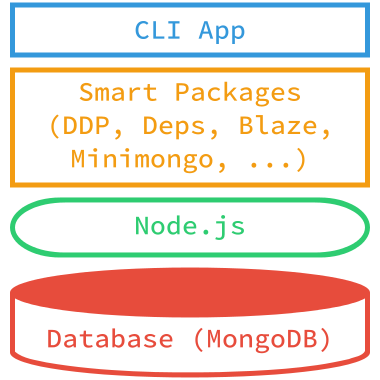
\includegraphics[width=4cm]{\dir/include/meteor-stack.png}
  \caption[Meteor Stack]{Meteor stack of tools/technologies}
  \label{fig:meteor-stack}
\end{figure}

Meteor in terms of application is both library of packages (pre-written and self-contained modules that needed) and command-line tools.
Like in \autoref{fig:meteor-stack}, the platform consists of three areas~\autocite{Hochhaus2014Meteor}:

\begin{description}
\item [Command line interface (CLI)] a hybrid between a build-tool and a package manager
\item [Collection of software] a suite of core packages provide functionality that can also be extended with custom packages or \ac{npm} modules
\item [Server infrastructure] both Node.js and MongoDB are an integral part of any Meteor installation
\end{description}

Beyond framework and platform, Meteor is also an integrated environment.
Since in the beginning of application development, it has a very tight coupling with \ac{DDP} and MongoDB.
So from there, we can do stuff faster without prior configuration over the protocol and database.
It can be run instantly then it just works.

\noindent There are seven principles that Meteor hold:

\begin{description}
\item [Data on the Wire] The server sends data and lets the client render it.
\item [Database Everywhere] The methods to access database from the client or the server are the same.
\item [One Language] The language to write both the client and the server parts of the application is only JavaScript.
\item [Latency Compensation] The client prefetches data and simulates models to make it look like server method calls return instantly.
\item [Full Stack Reactivity] The interaction is realtime by default. All layers, from database to template, update themselves automatically when necessary.
\item [Embrace the Ecosystem] The platform is open source and integrates with existing open source tools and frameworks.
\item [Simplicity Equals Productivity]  The main functionality has clean, classically beautiful APIs.
\end{description}

Meteor has a \ac{CLI} installer that officially supports Linux on \verb|x86| and \verb|x86_64| architectures, also Mac OS X $10.7$ and above.
How install the Meteor with one command on Linux or OS X terminal is just with:

\begin{verbatim}
curl https://install.meteor.com | sh
\end{verbatim}

\noindent Then create a basic app just like:

\begin{verbatim}
meteor create app-name
\end{verbatim}

This created these files (\ac{HTML}, \ac{CSS}, \ac{JS}, and Meteor files) with a sample code into the \verb|app-name| directory:

\begin{verbatim}
app-name.js
app-name.html
app-name.css
.meteor
\end{verbatim}

To run it, simply go to the app directory and run Meteor:

\begin{verbatim}
cd app-name
meteor
\end{verbatim}

By default, it runs the app via \ac{URL} \verb|http://localhost:3000| and can be run via browser.
If there is an edit in one or some of the files, Meteor will rebuild and update the app automatically with the new code and content.
\noindent Below listing \autoref{lst:meteor-html}, \autoref{lst:meteor-js}, and \autoref{lst:meteor-css} are the actual source code of a very basic Meteor application that built with those commands.

\begin{listing}[!hp]
\caption{View (HTML) part of Meteor}
\inputminted{html}{\dir/include/meteor/meteor.html}
\label{lst:meteor-html}
\end{listing}

\begin{listing}[!hp]
\caption{Logic (JavaScript) part of Meteor}
\inputminted{javascript}{\dir/include/meteor/meteor.js}
\label{lst:meteor-js}
\end{listing}

\begin{listing}[!hp]
\caption{Style (CSS) part of Meteor}
\inputminted{css}{\dir/include/meteor/meteor.css}
\label{lst:meteor-css}
\end{listing}
